\chapter{Parallelization}

Here we describe full parallelization of the previous 
algorithm. The fully parallelized code can be seen in appendix A.

\section{Process}

The main process of the algorithm as described by dataflow.\cite{Kahn74,Lee95}

\begin{figure}[H]
	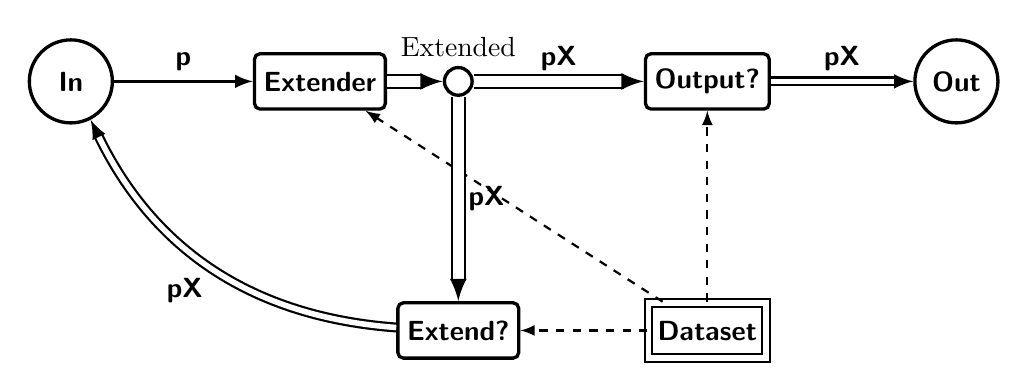
\begin{tikzpicture}[auto]
	\tikzstyle{pool} = [
		draw, very thick, fill=white, 
		circle,
		minimum height=3em, minimum width=3em, 
		node distance=9em, font={\sffamily\bfseries}];
	\tikzstyle{temppool} = [
		draw, very thick, fill=white, 
		circle,
		minimum height=1em, minimum width=1em, 
		node distance=5em, font={\sffamily\bfseries}];

	\tikzstyle{filter} = [
		draw, very thick, fill=white, 
		rectangle, rounded corners=0.2em,
		minimum height=2em, minimum width=4em,
		node distance=9em, font={\sffamily\bfseries}];
	\tikzstyle{extender} = [
		draw, very thick, fill=white, 
		rectangle, rounded corners=0.2em,
		minimum height=2em, minimum width=4em,
		node distance=9em, font={\sffamily\bfseries}];

	\tikzstyle{dataset} = [
		draw, thick, fill=white, 
		rectangle, double, double distance=2pt,
		minimum height=2em, minimum width=4em,
		node distance=9em, font={\sffamily\bfseries}];

	\tikzstyle{take} = [
		very thick, ->, >=latex,
		text centered, font={\sffamily\bfseries}];
	\tikzstyle{chan} = [
		thick, ->, >=latex, double, double distance=4pt,
		text centered, font={\sffamily\bfseries}];
	\tikzstyle{filtered} = [
		thick, ->, >=latex, double, double distance=2pt,
		text centered, font={\sffamily\bfseries}];
	\tikzstyle{needs} = [
		thick, ->, >=latex, dashed,
		text centered, font={\sffamily\bfseries}];

	\node[pool] (in) {In};
	\node[extender, right of=in] (ext) {Extender};
	\node[temppool, right of=ext, label=above:Extended] (exts) {};
	\node[filter, right of=exts] (outable) {Output?};
	\node[filter, below of=exts] (extable) {Extend?};
	\node[pool, right of=outable] (out) {Out};

	\node[dataset, right of=extable] (dataset) {Dataset};
	\draw[needs] (dataset) to (ext);
	\draw[needs] (dataset) to (outable);
	\draw[needs] (dataset) to (extable);

	\draw[take] 
		(in) to node{p} (ext);
	\draw[chan]
		(ext) to (exts);
	\draw[chan] 
		(exts) to node{pX} (outable);
	\draw[chan] 
		(exts) to node{pX} (extable);
	\draw[filtered, bend left] 
		(extable) to node{pX} (in);
	\draw[filtered]
		(outable) to node{pX} (out);
\end{tikzpicture}

\end{figure}

The easiest thing here to parallelize is the extender since it's interaction
can be seen as a separate unit.

\section{Adding Nodes}

If instead of in/out pool we had several the algorithm can still work, if we
have single take / put process to decide which actual pool to use.

We can use several extenders that work in parallel without problems since they do not need information about other querys nor input/output pools.

\section{Extending}

We still can also do the extending process in parallel:

\begin{verbatim}
func extender(query) {
	// find all next positions
	nexts = (map next query.matches)
	matches = (group nexts by token)
	result = (map newquery matches)
	other = (map #(union (matches %1)) groups)
	return result union other
}
\end{verbatim}

\section{Dataset partitioning}

If we look at where we need synchronization points if we partition the dataset. Whole parts of extension still apply for parts of dataset.

Synchronization is only needed for filtering. We don't need to know the whole query but just information about parts to make a decision whether to filter or not.

\section{Filtering}

This is the only place where we may need the whole information about the query.

Although many operations can be parallelized with map reduce.

\todo[inline]{example how to do counting}

\todo[inline]{example what cannot be done easily on sharded data}